\chapter{Data augmentation}\label{data-augmentation}

Con Data augmentation si intende la tecnica usata per la generazione di nuovi dati  al fine di aumentare artificialmente il numero di campioni di allenamento ed è diventato una pratica comune nell'area del deep learning.

È noto che l'aumento dei dati può aumentare l'invarianza di un classificatore e può agire come un regolatore nel prevenire l'overfitting nelle reti neurali, come in AlexNet (la rete utilizzata in questa tesi). Gli autori del noto AlexNet  hanno dichiarato che senza l'aumento dei dati la loro rete avrebbe sofferto di un sostanziale overfitting, che li avrebbe costretti a usare reti meno profonde \cite{alexnet}. Ma non solo le reti profonde, anche quelle meno profonde  possono essere notevolmente migliorate adottando l'aumento dei dati \cite{dataaugmentation}.


\section{Metodi comuni di Data augmentation}\label{metodi-comuni-di-data-augmentation}

Le principali operazioni sono per esempio  il ritaglio di immagini
per l'addestramento in posizioni diverse, la rotazione delle immagini (sia leggere di qualche grado che di 90, 180, 240 gradi), ecc. Queste trasformazioni geometriche usate per modificare la disposizione spaziale dei pixel in una 
immagine sono anche chiamate trasformazioni rubber-sheet (foglio malleabile) perché 
possono essere viste come analoghe alla "stampa" di un'immagine su un foglio malleabile dove è possibile stirarlo e piegarlo. La trasformazione delle coordinate può essere espressa come:
\[ \left[\begin{array}{l}x^{\prime} \\ y^{\prime}\end{array}\right]=\symbfup{T}\left[\begin{array}{l}x \\ y\end{array}\right]=\left[\begin{array}{ll}t_{11} & t_{12} \\ t_{21} & t_{22}\end{array}\right]\left[\begin{array}{l}x \\ y\end{array}\right] \]
Dove \((x,y)\)  sono le coordinate dei pixel nell'immagine originale, \((x^{\prime},y^{\prime})\)  le 
coordinate dei pixel corrispondenti dell'immagine trasformata, \(\symbfup{T}\) la matrice di trasformazione, per poter effettuare tutte le trasformazioni rubber-sheet è necessario usare un piano affine che aggiunga una dimensionalità:
\[ \left[\begin{array}{l}x^{\prime} \\ y^{\prime} \\ 1\end{array}\right]=\symbfup{A}\left[\begin{array}{l}x \\ y \\ 1\end{array}\right]=\left[\begin{array}{ccc}a_{11} & a_{12} & a_{13} \\ a_{21} & a_{22} & a_{23} \\ 0 & 0 & 1\end{array}\right]\left[\begin{array}{l}x \\ y \\ 1\end{array}\right] \]

In questo caso la matrice \(\symbfup{A}\) è la nostra matrice affine di trasformazione, che può scalare, ruotare o specchiare un'immagine, una DA basica da applicare a una rete neurale è la seguente \cite{nanni_dct_pca} \cite{gonzalez_dip}:
\begin{itemize}
    \item L'immagine si riflette nella direzione sinistra-destra con il 50\% di probabilità. La matrice di trasformazione \(\symbfup{A}\) è:
    \[\symbfup{A} = \left[\begin{array}{lll}\pm 1 & 0 & 0 \\ 0 & 1 & 0 \\ 0 & 0 & 1\end{array}\right]\]
    \item L'immagine è riflessa in modo casuale in entrambe le direzioni sinistra-destra e in alto-basso.
    \[\symbfup{A} = \left[\begin{array}{lll}1 & 0 & 0 \\ 0 & \pm 1 & 0 \\ 0 & 0 & 1\end{array}\right]\]
    \item Dalla trasformazione precedente l'immagine viene scalata lungo entrambi gli assi di due diversi fattori che sono
    campionati casualmente dalla distribuzione uniforme tra \([1...2]\).
    \[\symbfup{A} = \left[\begin{array}{lll}\pm z_x & 0 & 0 \\ 0 & \pm z_y & 0 \\ 0 & 0 & 1\end{array}\right] \quad z_x, z_y \sim U(1,2)\]
    \item Combina tutte le trasformazioni precedenti  e aggiunge la rotazione e la traslazione dell'immagine in entrambe le
    direzioni. La rotazione viene effettuata utilizzando un angolo che viene campionato casualmente dall'intervallo
    \([-10...10]\), mentre la traslazione consiste nello spostare l'immagine di un certo numero di pixel
    campionati casualmente da \([0...5]\).
    \[\symbfup{A} = \left[ \begin{array} { lll } \cos \theta & - \sin \theta & 0 \\ \sin \theta & \cos \theta & t_x \\ 0 & t_y & 1 \end{array} \right] \quad z_x, z_y \in U(1,2) \quad \theta \sim U(-10,10) \quad t_x, t_y \sim U(0,5)\]
\end{itemize}

\section{Data augmentation con DCT}\label{data-augmentation-con-dct}

In aggiunta alle trasformazioni standard precedenti si usa anche l'approccio trattato in  \cite{nanni_dct_pca} attraverso le modifiche nei sottospazi ottenuti tramite le trasformazioni Discrete Cosine
Transform (DCT). La trasformazione è basata sulla proiezione dell'immagine originale sul sottospazio DCT, sulla perturbazione del sotto spazio e dalla proiezione dell'immagine perturbata dal sottospazio al dominio immagine, come mostrato in \cref{fig:dct-schema}.

\begin{figure}[ht]
    \centering
    
\includegraphics[width=1\textwidth]{data-augmentation/dct-trasformazione.pdf}
    \caption{Architettura di una trasfromazione via DCT}
    \label{fig:dct-schema}
\end{figure}


\section{Discrete Cosine Transform (DCT)}\label{discrete-cosine-transform-dct}


La Discrete Cosine Transform è una delle più importanti trasformate nell'ambito della computer vision, in particolare è in grado di rilevare le  variazioni di informazione tra un'area e quella contigua di un'immagine raster trascurando le ripetizioni. Viene usata in numerosi ambiti dalla compressione delle immmagini all'elaborazione delle immagini. In particolare è simile alla  trasformata discreta di Fourier (DFT), ma fa uso solo di numeri reali, in particolare la DCT tipo I è definita come \cite{syed_dct} \cite{gonzalez_dip}:

\[ \operatorname{DCT}(x)=\alpha(x) \sum_{p=1}^{n} f(p) \cos \left(\frac { \pi p  (x- 1) } { 2 n }\right) \]

Per ogni \(x\in [0...n]\) con \(n\) dimensione dell'immagine. Dove \(\alpha(n)\) è definita come:
\[\alpha(n) = \left\{ \begin{array} { l } \sqrt { \frac { 1 } { n } } , n = 1 \\ \sqrt { \frac { 2 } { n } } , n > 1 \end{array} \right.\]

Similmente la trasformazione inversa è definita come \cite{syed_dct}:

\[\operatorname{IDCT}(x)=\sum^{n}_{p=1} \alpha(p)\operatorname{DCT}(p) \cos \left(\frac { \pi p  (x- 1) } { 2 n }\right)\]


Ci sono numerose varianti della DCT, in particolare la DCT tipo I che è la definizione mono dimensionale della DCT; la DCT tipo II, che spesso è chiamata DCT e la sua inversa: la DCT tipo III che viene chiamata spesso come la IDCT. In linguaggio matematico la formula della DCT tipo II è la seguente \cite{syed_dct} \cite{gonzalez_dip} \cite{nanni_dct_pca}:


\[\operatorname{DCTimage} ( x , y ) = \alpha( x ) \alpha (y) \sum _ { \mathclap{(p , q) = (1,1)} } ^ { \mathclap{(n,m)} }  \operatorname { Image } ( p , q ) \cos \left(\frac { \pi p  (x-1) } { 2 n }  \right) \cos \left(\frac { \pi q  (y-1) } { 2 m }  \right) \]

Per ogni \((x,y) \in [0..n]\times [0...m]\), dove \(n,m\) rappresentano la dimensione dell'immagine. Similmente la DCT tipo III o IDCT è definita come \cite{syed_dct} \cite{gonzalez_dip}:

\[\operatorname{IDCTimage} ( x , y ) = \sum _ { \mathclap{(p , q) = (1,1) }} ^ {  \mathclap{(n,m) }} \alpha( p ) \alpha (q) \operatorname { DCTimage } ( p , q ) \cos \left(\frac {  \pi p  (x-1) } { 2 n }  \right) \cos \left(\frac { \pi q  (y-1) } { 2 m }  \right) \]

In particolare si individuano 2 possibili algoritmi di preprocessing DCT, che sono illustrati in \cref{fig:dct-algoritmi}.
\begin{figure}[ht]
    \centering
    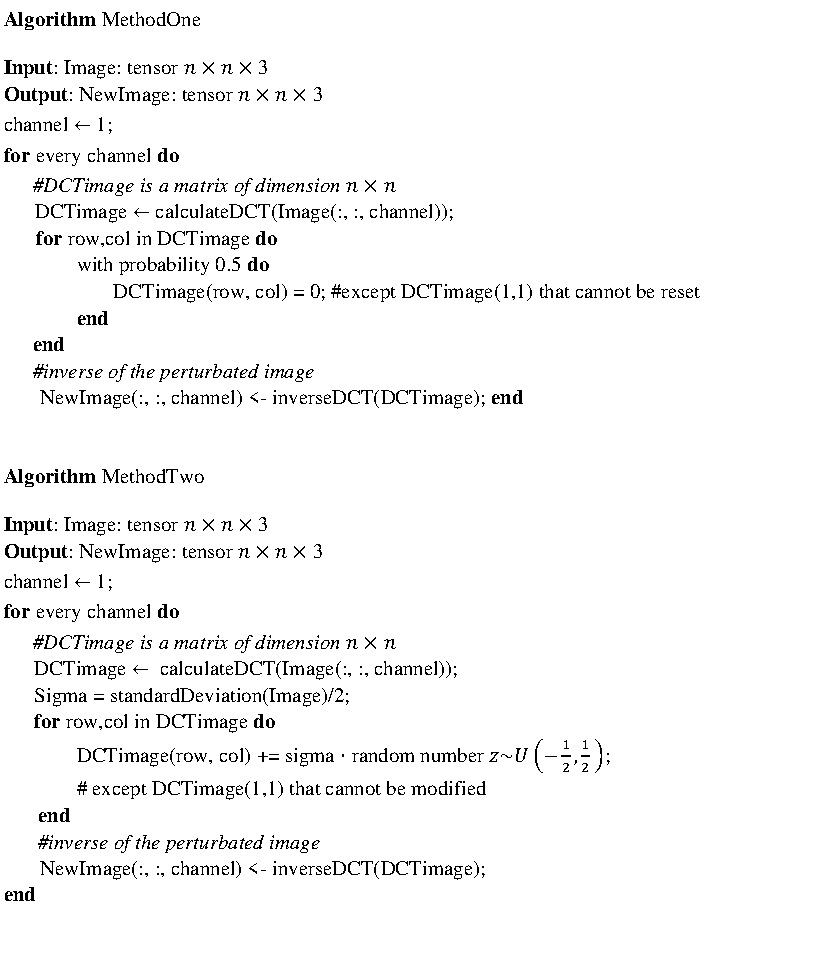
\includegraphics[width=1\textwidth]{addestramento-rete-neurale/Algorithm-MethodDCT.pdf}
    \caption{Due algoritmi di data augmentation con DCT}
    \label{fig:dct-algoritmi}
\end{figure}
